\chapter{Introduction}
Analysis of RADAR systems in maritime environments is complicated by the fact that the ocean does not generally provide a smooth or uniform surface to work with. Altitude variations change the aspect angle for multipath bounces, cause wave blockage, and add clutter and spikes to the echo return \cite{skolnik_handbook}, \cite{blake_radar}, \cite{nathanson_radar}. These are random, not deterministic effects which in turn induce signal fluctuations that have a significant impact on the probability of detecting a target. Understanding the impact of the sea surface on propagation is critical to evaluating the performance of a RADAR system in a maritime environment.

When we look at cases where the transmitter and receiver are not colocated, we have a bistatic configuration and analyzing performance becomes even more difficult \cite{willis_bistatic}. We cannot leverate reciprocity as paths are no longer constant, and the effects of multipath and clutter are often skewed. With multiple receivers or transmitters, the configuration is termed multistatic as there are multiple bistatic elements. Of particular concern here is the case with a single transmitter and multiple receivers.

\section{Objective}
The objective of this work is to evaluate the performance of multistatic RF sensor networks and demonstrate that Random Matrix Theory (RMT) allows prediction of the signal statistics. This will be accomplished in several phases. First, the ocean surface will be modeled in 2-dimensions to ensure that the appropriate ocean wave statistics are captures with the correct correlations in both the down range and cross range directions. Second, a Monte Carlo study will be performed to generate RADAR signal statistics. This study will be executed by generating a series of sea surfaces and then numerically propagating a RADAR signal through a Parabolic Wave Equation solver. The study will cover multiple sea states and geometric configurations. Finally, RMT will be used to generate a statistical model that encompasses the results.

\section{Multistatic RF Sensor Network Concept}
An example multistatic RF sensor network in a maritime environment is shown in Figure \ref{ms_fig:1}. In this concept, a single transmitter illuminates a target and the echo signal is captured by a pair of receivers. The received signal will fluctuate due to multipath reflections from the surface, path variations, and relative motion of the target. In addition, each receiver observes the target from a different aspect angle than it was illuminated with, resulting in different radiation patterns.

\begin{figure}[H]
  \begin{center}
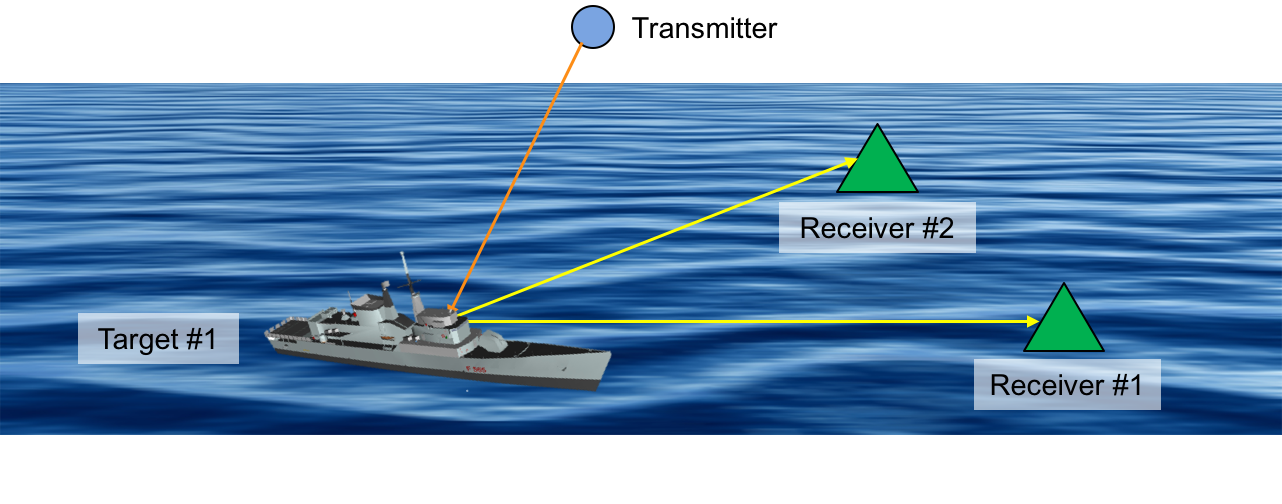
\includegraphics[width=5in]{../media/multistatic/ms_rf_concept.png}
  \end{center}
  \renewcommand{\baselinestretch}{1} \small\normalsize
  \begin{quote}
    \caption[Multistatic RF Sensor Networks Concept]{Multistatic RF Sensor Networks Concept\label{ms_fig:1}}
  \end{quote}
\end{figure}
\renewcommand{\baselinestretch}{2} \small\normalsize
